%%%%%%%%%%%%%%%%%%%% book.tex %%%%%%%%%%%%%%%%%%%%%%%%%%%%%
%
% sample root file for the chapters of your "monograph"
%
% Use this file as a template for your own input.
%
%%%%%%%%%%%%%%%% Springer-Verlag %%%%%%%%%%%%%%%%%%%%%%%%%%


% RECOMMENDED %%%%%%%%%%%%%%%%%%%%%%%%%%%%%%%%%%%%%%%%%%%%%%%%%%%
\documentclass[pdftex,12pt, oneside]{article}

% choose options for [] as required from the list
% in the Reference Guide, Sect. 2.2
%\usepackage[paperwidth=8.5in, paperheight=13in]{geometry} % Folio
\usepackage[paperwidth=8.27in, paperheight=11.69in]{geometry} % A4

\usepackage{makeidx}         % allows index generation
\usepackage{graphicx}        % standard LaTeX graphics tool
                             % when including figure files
%\usepackage{multicol}        % used for the two-column index
\usepackage[bottom]{footmisc}% places footnotes at page bottom
\usepackage[bahasa]{babel}
\usepackage{enumerate}
\usepackage{paralist}
\usepackage{float}
\usepackage{gensymb}  
\usepackage{listings}
\usepackage{hyperref}
%\usepackage{siunitx}
% etc.
% see the list of further useful packages
% in the Reference Guide, Sects. 2.3, 3.1-3.3
\renewcommand{\baselinestretch}{1.5}

\newcommand{\HRule}{\rule{\linewidth}{0.5mm}}

%\makeindex             % used for the subject index
                       % please use the style svind.ist with
                       % your makeindex program


%%%%%%%%%%%%%%%%%%%%%%%%%%%%%%%%%%%%%%%%%%%%%%%%%%%%%%%%%%%%%%%%%%%%%

\begin{document}

%\input{./01.title.tex}
\begin{center}
{\large STUDI KELAYAKAN SISTEM KOMPUTER UNTUK PEMBANGUNAN LAYANAN SISTEM OTENTIKASI DI BADAN PENGELOLAAN PENDAPATAN, KEUANGAN DAN ASET DAERAH KABUPATEN BREBES}
\\[1cm]
20 Februari 2019\\
Priyanto Tamami, S.Kom.
\end{center}

\section{RUANG LINGKUP PEKERJAAN}

Ruang lingkup dari pekerjaan studi kelayakan sistem komputer ini hanya sebatas menilai apakah sistem komputer yang sudah ada layak atau tidak untuk digunakan sebagai basis layanan sistem otentikasi di Badan Pengelolaan Pendapatan, Keuangan dan Aset Daerah Kabupaten Brebes.

Aplikasi atau sistem otentikasi yang akan dibangun diatas sistem komputer ini nantinya akan dibangun berbasis \textit{web}, sehingga dari sisi peladen (\textit{server}) nantinya, sistem komputer yang terpasang harus mampu baik secara perangkat keras (\textit{hardware}) maupun perangkat lunak (\textit{software}), memberikan layanan bagi setiap komputer klien yang terpasang baik di kantor maupun di masyarakat umum. Sedangkan dari sisi komputer klien, lingkupnya hanya sebatas komputer klien yang terdapat di bidang Pendataan dan Penetapan pada Badan Pengelolaan Pendapatan, Keuangan dan Aset Daerah Kabupaten Brebes, apakah sistem komputer yang terpasang, baik secara perangkat keras (\textit{hardware}) dan perangkat lunaknya (\textit{software}) mampu untuk melakukan akses ke peladen (\textit{server}) dari layanan (\textit{service}) \textit{OAuth Server}.

Karena aplikasi yang dibangun di atas sistem komputer di sisi peladen (\textit{server}) ini akan berbasis \textit{container} docker, tentunya perangkat lunak docker wajib terpasang, sedangkan di sisi komputer klien, yang dibutuhkan hanyalah sebuah peramban (\textit{browser}) untuk melakukan akses ke layanan di sisi peladen (\textit{server}).

Hal-hal yang mendukung studi kelayakan sistem komputer yang dibutuhkan oleh sistem otentikasi di Badan Pengelolaan Pendapatan, Keuangan dan Aset Daerah ini yaitu dengan menggunakan metode analisis kelayakan TELOS (\textit{Technical}, \textit{Economic}, \textit{Legal}, \textit{Operational}, \textit{Schedule}).

Detail dari masing-masing faktor pada metode analisis kelayakan TELOS ini adalah seperti berikut :

\begin{enumerate}
	\item Faktor Kelayakan Teknis (\textit{Technical})
	
Kelayakan teknis menyoroti kebutuhan sistem yang telah disusun dari aspek teknologi yang digunakan, jika teknologi yang dikehendaki untuk pengembangan sistem merupakan teknologi yang mudah didapat, murah, dan tingkat pemakaiannya mudah, maka secara teknis usulan kebutuhan sistem bisa dinyatakan layak.

	\item Faktor Kelayakan Ekonomi (\textit{Economic})
	
Aspek yang paling dominan dari aspek kelayakan yang lain adalah kelayakan ekonomi. Tidak dapat disangkal lagi, motivasi pengembangan sistem informasi pada perusahaan atau organisasi adalah motif keuntungan. Dengan demikian aspek untung rugi jadi pertimbangan utama dalam pengembangan sistem, termasuk di dalamnya adalah kelayakan ekonomi atas sistem komputer yang akan digunakan. Kelayakan ekonomi berhubungan dengan \textit{return investmen} atau berapa lama biaya investasi dapat kembali, namun pada instansi pemerintah, yang secara umum bertugas melayani masyarakat, maka hubungannya bukan lagi untung rugi, tetapi lebih kepada imbas administrasi data yang tercatat dengan baik dan sedikit banyak mungkin berpengaruh pada peningkatan kepatuhan wajib pajak dalam memenuhi kewajiban pajaknya.	

	\item Faktor Kelayakan Hukum (\textit{Legal})
	
Menguraikan secara hukum apakah sistem komputer yang dibutuhkan tidak menyimpang dari hukum yang berlaku (tidak melanggar hukum jika diterapkan di objek penelitian). Misal: bagaimana kelayakan perangkat lunak yang digunakan, bagaimana kelayakan hukum informasi yang dihasilkan oleh program aplikasi yang dibuat. Apakah melanggar hukum atau tidak.	

	\item Faktor Kelayakan Operasional (\textit{Operational})

Penilaian terhadap kelayakan operasional digunakan untuk mengukur apakah sistem yang akan dikembangkan nantinya dapat dioperasikan dengan baik atau tidak untuk melayani kebutuhan otentikasi dan otorisasi.	

	\item Faktor Kelayakan Jadwal (\textit{Schedule})
	
Penilaian kelayakan jadwal ini digunakan untuk menentukan bahwa pengembangan sistem akan dapat dilakukan dalam batas waktu yang telah ditetapkan.	

\end{enumerate}

Adapun penilaian untuk masing-masing faktor kelayakan TELOS ini adalah sebagai berikut :

\begin{enumerate}
	\item Menilai kelayakan Teknik (\textit{Technical})

Kelayakan teknik menyoroti kebutuhan sistem yang telah disusun dari teknologi yang akan digunakan, untuk penerapan sistem otentikasi di Badan Pengelolaan Pendapatan, Keuangan dan Aset Daerah. Sistem ini merupakan sistem berbasis layanan otentikasi yang digunakan oleh aplikasi yang akan dibangun yang datanya menggunakan data-data Pajak Daerah dan akses datanya terbatas untuk tiap jabatan pengguna, sehingga di masa mendatang, aplikasi yang dibangun tidak memerlukan bagian otentikasi, proses otentikasi cukup diserahkan ke sistem OAuth yang akan dibangun ini.

Sistem ini nantinya akan menerima permintaan sebuah token dari aplikasi klien, yang apabila belum pernah masuk sama sekali, sistem akan menampilkan halaman masuk (\textit{login}) untuk memastikan bahwa pengguna (\textit{end-user}) sudah terdaftar dan memiliki hak untuk melakukan akses data. Apabila proses \textit{login} telah berhasil, maka aplikasi klien akan mendapatkan sebuah token yang dapat digunakan untuk melakukan akses data ke \textit{resource server}.

Token yang diberikan oleh \textit{OAuth server} berbentuk JWT (\textit{JSON Web Token}) yang akan digunakan oleh aplikasi klien melakukan akses ke \textit{resource server}. Token dalam bentuk JWT ini sebetulnya sudah memiliki informasi yang cukup bagi aplikasi klien melakukan pengaturan akses bagi pengguna yang sedang melakukannya, tentunya aplikasi klien perlu melakukan \textit{decode} terlebih dahulu pada JWT yang diterima dari \textit{OAuth Server}.

Token dalam bentuk JWT ini wajib selalu dikirimkan oleh aplikasi klien pada saat melakukan akses ke \textit{resource server}, hal ini untuk memastikan bahwa data yang berada di \textit{resource server} diakses oleh pengguna yang memiliki hak.

\begin{enumerate}
	\item Kebutuhan Perangkat Keras, Perangkat Lunak, dan Perangkat Jaringan
	
\begin{enumerate}
	\item Perangkat Keras
	
Kebutuhan akan perangkat keras, sebetulnya tidak diperlukan pengadaan alat baru, melainkan dengan menggunakan perangkat yang sudah ada, sistem informasi ini akan dapat berjalan sebagaimana mestinya. Adapun perangkat keras yang digunakan adalah seperti berikut :

\begin{table}[H]
\centering
\begin{tabular}{| c | l | l |}
\hline
No & Perangkat keras & Keterangan \\
\hline
\multicolumn{3}{| c |}{\textit{Server} Aplikasi} \\
\hline
1 & Prosesor & Intel Xeon 2,4G 8 Core\\
\hline
2 & Memori & 8 GB \\
\hline
3 & Harddisk & \\
\hline
4 & Jaringan & 4 ethernet slot \\
\hline
\multicolumn{3}{| c |}{\textit{Server} Basis Data} \\
\hline
1 & Prosesor & Intel Xeon 2,4G 8 Core \\
\hline
2 & Memori & 32 GB \\
\hline
3 & Harddisk & \\
\hline
4 & Jaringan & 4 ethernet slot \\
\hline
\end{tabular}
\end{table}

	\item Perangkat Lunak
	
Kebutuhan akan perangkat lunak baru tentunya ada, tetapi tidak memerlukan biaya tambahan, karena beberapa perangkat lunak ada yang sudah terpasang, dan perangkat lunak yang akan di\textit{install} tidak memerlukan biaya tambahan.

\begin{table}[H]
	\centering
	\begin{tabular}{| c | l | l |}
		\hline
		No & Perangkat Lunak & Kegunaan \\
		\hline
		1 & Windows Server 2008 & Sistem Operasi \\
		\hline
		2 & Linux Ubuntu & Sistem Operasi \\
		\hline
		3 & IntelliJ IDEA & IDE \\
		\hline
		4 & Visual Studio Code & Editor \\
		\hline
		5 & Docker & Container \\
		\hline
		6 & Chrome, Firefox & Web Browser \\
		\hline
	\end{tabular}
\end{table}	

	\item Perangkat Jaringan
	
Kebutuhan akan perangkat jaringan pun tidak memerlukan pengadaan kembali, karena kondisi jaringan sudah terhubung dengan baik dengan peralatan seperti berikut :

\begin{table}[H]
	\centering
	\begin{tabular}{| c | l | l |}
		\hline
		No & Perangkat & Kegunaan \\
		\hline
		1 & Switch & Penghubung antar kabel jaringan \\ 
		\hline 
		2 & Kabel UTP & Media penghubung antar perangkat \\
		\hline
		3 & Konektor RJ-45 & Media penghubung antara kabel dengan \textit{socket} perangkat \\
		\hline
		4 & Modem & Sebagai perangkat penghubung jaringan lokal dan internet \\
		\hline
		5 & Router & Penghubung antar 2 atau lebih jaringan (berdasarkan alamat jaringan) \\
		\hline
	\end{tabular}
\end{table}	
	
\end{enumerate}	

	\item Arsitektur Jaringan Komputer
	
Arsitektur jaringan sistem informasi ini adalah seperti pada gambar \ref{fig:001-arsitektur-sistem}. Bila ada seorang pengguna yang melakukan akses dengan \textit{browser}, maka akan ditampilkan halaman utama dari sistem informasi ini. 

\begin{figure}[H]
	\centering
	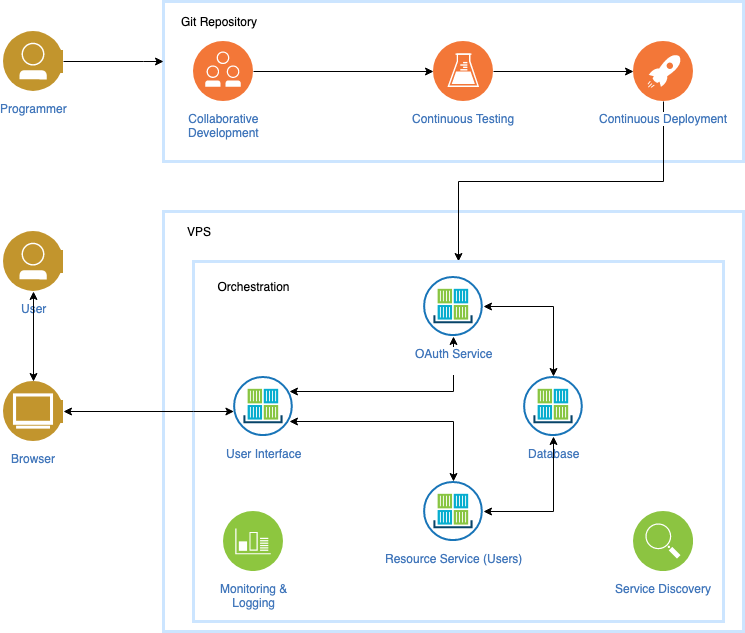
\includegraphics[width=1\textwidth]{./resources/arsitektur-sistem}
	\caption{Desain Arsitektur Sistem}
	\label{fig:001-arsitektur-sistem}
\end{figure}

Nantinya, saat pengguna akan melakukan akses terhadap beberapa aplikasi yang terproteksi, pengguna akan diarahkan ke halaman \textit{login} milik \textit{OAuth Service} untuk mengisikan \textit{username} dan \textit{password}. 

Setelah proses otentikasi berhasil dilakukan, selanjutnya halaman pada peramban (\textit{browser}) akan dikembalikan ke halaman aplikasi yang akan diakses, dimana proses yang berjalan dibelakang layar adalah \textit{OAuth Service} akan memberikan sebuah \textit{token} ke aplikasi klien untuk disimpan dan digunakan setiap akan melakukan proses permintaan data (\textit{request}) ke \textit{Resource Service}. 

Selanjutnya, saat pengguna akan melakukan akses data melalui halaman aplikasi \textit{web} klien, aplikasi ini akan melakukan permintaan (\textit{request}) data ke \textit{resource service} dengan membawa data dan \textit{token}, yang kemudian \textit{resource service} akan melakukan verifikasi hak akses melalui \textit{token} tersebut, apabila hak akses tidak sesuai, maka akan mengembalikan pesan kesalahan bahwa permintaan atau \textit{request} tersebut tidak dapat dipenuhi, namun bila hak aksesnya sesuai, maka data akan dikirimkan ke aplikasi klien untuk ditampilkan ke pengguna.

\end{enumerate}

Adapun kondisi sistem informasi yang digunakan saat ini adalah seperti berikut :

\begin{enumerate}
	\item Sistem Aplikasi 
	
Aplikasi adalah sebuah \textit{tools} untuk membantu dan mempermudah suatu aktifitas administrasi maupun yang lainnya. Tanpa adanya aplikasi, tentu suatu aktifitas tidak bisa diselesaikan dengan cepat, segala sesuatunya dilakukan dengan pencatatan manual. Aplikasi atau sistem informasi yang digunakan di Bidang Pendataan dan Penetapan pada Badan Pengelolaan Pendapatan, Keuangan dan Aset Daerah Kabupaten Brebes saat ini adalah :

\begin{table}[H]
	\centering
	\begin{tabular}{| c | l | l |}
		\hline
		No & Aplikasi & Keterangan \\
		\hline
		1 & SISMIOP & Melakukan manajemen objek pajak PBB-P2 \\
		\hline
		2 & Simda Pendapatan & Melakukan pengelolaan pajak daerah \\
		\hline
		3 & Microsoft Excel & Digunakan untuk merekam dan mengolah data peralihan hak \\
		\hline
	\end{tabular}
\end{table}

Dengan adanya sistem informasi atau aplikasi SISMIOP, sudah membantu pengelolaan pajak daerah untuk jenis Pajak Bumi dan Bangunan sektor Perdesaan dan Perkotaan dari mulai manajemen pelayanan, pendataan,  penetapan, penagihan, hingga ke prosedur pembayaran.

Sedangkan aplikasi Simda Pendapatan, sudah dapat membantu melakukan pengelolaan pajak daerah untuk jenis pajak selain Pajak Bumi dan Bangunan sektor Perdesaan dan Perkotaan, namun belum sepenuhnya dapat melakukan pengelolaan yang terjadi pada jenis Bea Perolehan Hak Atas Tanah dan Bangunan.

Dengan semakin bertambahnya kebutuhan organisasi akan aplikasi atau sistem informasi kedepan, maka akan semakin bertambah pula otentikasi dan otorisasi untuk tiap penggunanya, untuk mengantisipasi kondisi seperti ini, maka kebutuhan untuk membangun sebuah sistem OAuth diperlukan sehingga nantinya tiap pengguna tidak perlu melakukan \textit{login} berulang-ulang untuk melakukan akses ke beberapa aplikasi yang terproteksi.

	\item Sistem Basis Data
	
Basis data merupakan suatu tempat penyimpanan data-data yang biasanya dari sebuah aplikasi, adapun basis data yang sudah ada pada Badan Pengelolaan Pendapatan, Keuangan dan Aset Daerah adalah seperti berikut :

\begin{table}[H]
	\centering
	\begin{tabular}{| c | l | l |}
		\hline
		No & Basis data & Keterangan \\
		\hline
		1 & Oracle DB & Digunakan untuk menyimpan data dari aplikasi SISMIOP \\
		\hline
		2 & SQL Server & Digunakan untuk menyimpan data dari aplikasi Simda Pendapatan \\
		\hline
	\end{tabular}
\end{table}	

Basis data yang digunakan masih belum terintegrasi dengan baik, karena penerimaan pembayaran pada SISMIOP belum dapat secara otomatis tercatat pada Simda Pendapatan. 

Sebetulnya sumber data yang digunakan pada pengelolaan Pajak Bumi dan Bangunan sektor Perdesaan dan Perkotaan ada pada 2 (dua) tempat, yang pertama berada di Badan Pengelolaan Pendapatan, Keuangan dan Aset Daerah Kabupaten Brebes, yang kedua berada di BPD Jateng.

Kondisi data yang berada di Badan Pengelolaan Pendapatan, Keuangan dan Aset Daerah berfungsi sebagai pendataan dan penetapan, namun realisasi pembayaran menggunakan data dari BPD Jawa Tengah. Selisih nilai antara 2 (dua) sumber data ini pasti terjadi, maka seharusnya dibutuhkan personil untuk melakukan pencocokan / rekonsiliasi data antara 2 (dua) sumber data tersebut agar data yang ditampilkan pada sistem informasi yang akan dibangun menjadi lebih lengkap.

Untuk membangun sistem OAuth nantinya membutuhkan sistem basis data yang tentunya terpisah dari sistem yang telah ada, pengunaan sistem basis datanya pun tidak memerlukan biaya tambahan karena menggunakan sistem basis data yang gratis dan sudah teruji kehandalannya. Basis data ini nantinya akan merekam daftar pengguna dan kata kuncinya (\textit{password}) termasuk statusnya apakah sebagai pengguna yang statusnya aktif, atau pengguna yang statusnya di non-aktifkan, yang artinya tidak dapat melakukan akses masuk ke data-data yang terproteksi.

Pada sistem basis data yang digunakan OAuth ini pun akan merekam data aplikasi klien yang terdaftar yang dijinkan melakukan akses ke \textit{resource server} yang terproteksi.

Dilihat dari sisi teknis sistem basis data yang akan digunakan cukup handal, terbukti dengan banyaknya perusahaan besar menggunakan basis data ini dan tersedia secara gratis, maka syarat kebutuhannya sangat mencukupi untuk membangun sistem OAuth.

	\item Infrastruktur
	
Infrastruktur merupakan sarana yang sangat dibutuhkan dalam sebuah aktifitas apapun termasuk aktifitas pengelolaan Pajak Daerah. Adapun infrastruktur yang ada pada Badan Pengelolaan Pendapatan, Keuangan dan Aset Daerah Bidang Pendataan dan Penetapan yaitu :

\begin{table}[H]
	\centering
	\begin{tabular}{| c | l | l |}
		\hline 
		No & Infrastruktur & Keterangan \\
		\hline
		1 & Komputer & Memiliki 13 komputer dan 4 \textit{server} \\
		\hline
		2 & Printer & Memiliki 4 \textit{printer multi-purpose}, 4 \textit{printer dot-matrix}, \\
		& & 3 \textit{printer line-matrix} \\
		\hline
		3 & Jaringan Internet & Memiliki 2 (dua) sumber internet, dengan 1 (satu) internet \\
		& & \textit{shared bandwidth} dan 1 (satu) internet \textit{dedicated} \\
		\hline
	\end{tabular}
\end{table}

Dari kondisi infrastruktur di atas, sebetulnya Badan Pengelolaan Pendapatan, Keuangan dan Aset Daerah secara infrastruktur, syarat kebutuhannya sangat mencukupi untuk membangun sistem OAuth yang dapat digunakan sebagai pendukung aplikasi yang akan dibangun kedepannya.

\end{enumerate}

Melihat kondisi teknis demikian, dimana sistem komputer yang telah ada dianggap mampu melakukan tugasnya untuk penerapan aplikasi atau sistem otentikasi, sehingga nilai kelayakan teknik yang dapat diberikan adalah 9.0.

	\item Menilai kelayakan Ekonomi (\textit{Economic})
	
Pembangunan sistem baru tentunya membutuhkan investasi ataupun dana yang tidak sedikit, untuk mendapatkan manfaat di masa yang akan datang, sumber daya dan sumber dana diperlukan dalam pembangunan sistem baru sebagai bentuk investasi.

Untuk menganalisis kelayakan ekonomi digunakan kalkulasi analisis biaya dan manfaat (\textit{cost benefit analysis}). Adapun tujuan dari analisis biaya dan manfaat adalah untuk memberikan gambaran kepada internal Badan Pengelolaan Pendapatan, Keuangan dan Aset Daerah, apakah manfaat yang diperoleh dari sistem baru "lebih besar" dibandingkan dengan biaya yang dikeluarkan. 

Pada analisis biaya dan manfaat ada beberapa metode kuantitatif yang digunakan untuk menemukan standar kelayakan proyek.

\textbf{Analisis Biaya dan Manfaat}

Untuk melakukan analisa biaya dan manfaat diperlukan dua komponen, yaitu komponen biaya dan komponen manfaat.

\begin{enumerate}
	\item Komponen Biaya
	
Biaya yang berhubungan dengan pembuatan sistem ini dapat diklasifikasikan ke dalam 3 (tiga) kategori utama, yaitu :

\begin{enumerate}
	\item Biaya pengadaan, yaitu biaya pembelian perangkat keras, yang digunakan pada awal pembuatan sistem, sebelum sistem dioperasikan.
	\item Biaya Pengembangan, yaitu biaya pembuatan perangkat lunak sistem yang meliputi biaya konsultasi, biaya tahap analisa sistem, biaya tahap desain sistem dan biaya tahap penerapan sistem.
	\item Biaya operasi dan biaya perawatan, yaitu biaya yang dikeluarkan untuk menjalankan sistem, yaitu biaya \textit{overhead}, biaya perawatan terhadap perangkat keras dan perangkat lunak.
\end{enumerate}	

	\item Komponen Manfaat.
	
Manfaat yang didapat dari sistem informasi diklasifikasi sebagai berikut :

\begin{enumerate}
	\item Keuntungan berwujud adalah keuntungan yang berupa penghematan atau peningkatan di dalam pengelolaan pajak daerah yang dapat diukur dalam bentuk satuan nilai uang. Keuntungan berwujud antara lain :
	
	\begin{enumerate}
		\item Pengurangan biaya cetak
		\item Pengurangan biaya operasi
		\item Pengurangan biaya perlengkapan
	\end{enumerate}
	
	\item Keuntungan tak berwujud, adalah keuntungan yang sulit atau tidak mungkin diukur dalam bentuk satuan uang. Keuntungan tersebut antara lain :
	
	\begin{enumerate}
		\item Peningkatan efisiensi waktu pengerjaan
		\item Peningkatan efektifitas pegawai
		\item Peningkatan pelayanan pajak daerah
	\end{enumerate}
\end{enumerate}	

Adapun metode untuk melakukan analisis biaya dan manfaat adalah :

\begin{enumerate}
	\item Metode Periode Pengembalian

Metode ini adalah uji kuantitatif yang digunakan untuk menghitung jangka waktu yang diperlukan untuk membayar kembali biaya investasi dalam pembuatan aplikasi yang telah dikeluarkan. Penilaian kelayakan untuk pengembalian 

\[periode = \frac{investasi}{proceed} x tahun \]

\begin{enumerate}
	\item Layak jika waktu pengembalian lebih kecil dari umur investasi
	\item Tidak layak jika waktu pengembalian lebih besar dari umur investasi.
\end{enumerate}

Perhitungan Periode Pengembalian adalah seperti berikut :

Nilai Investasi = Rp0,-
Proses Th 1 = Rp100.364.100.000,-

Nilai investasi memang bernilai 0 (nol) rupiah karena seluruh sarana dan prasarana telah tersedia, hanya tinggal membangun sebuah sistem informasi untuk digunakan dan dijalankan. Sedangkan nilai Rp100.364.100.000,- (Seratus milyar tiga ratus enam puluh empat juta seratus ribu) didapat dari nilai target penerimaan untuk seluruh jenis Pajak Daerah di Kabupaten Brebes.

\[ PP = \frac{0}{100.364.100.000} \]

\[ PP = 0 tahun \]

Artinya, karena nilai investasi yang dikeluarkan nihil sama sekali, atau dengan kata lain tidak memerlukan nilai investasi, namun sistem informasi secara tidak langsung memberikan andil terhadap realisasi sebesar kurang lebih 100 Milyar Rupiah kepada Kas Daerah. Artinya sistem ini sangat layak untuk dikembangkan karena pengembalian tidak membutuhkan waktu untuk mencapai titik impas.

	\item Metode Pengembalian Investasi
	
Metode pengembalian investasi digunakan untuk mengukur presentase manfaat yang dihasilkan proyek dibandingkan dengan biaya yang dikeluarkan.

\textit{Return On Investmen} (ROI) dari suatu proyek dapat dihitung dengan rumus penilaian kelayakan untuk ROI :

\begin{enumerate}
	\item Layak jika ROI $>$ 0
	\item Tidak layak jika ROI $<$ 0
\end{enumerate}	

\[ ROI = \frac{Total Manfaat - Total Biaya}{Total Biaya} x 100\% \]
	
Karena nilai biaya tidak akan pernah muncul, maka bisa disebut bahwa Total Biaya = 0 (nol), Total Manfaat adalah penerimaan realisasi untuk seluruh jenis pajak daerah dalam satu tahun pajak, yaitu senilai 100.364.100.000 rupiah. Maka hasil yang didapatkan adalah seperti berikut :

\[ ROI = \frac{100.364.100.000 - 0}{0} x 100\% \]

\[ ROI = \infty \]

Ternyata karena kondisi pembaginya adalah 0 (nol), maka hasil yang didapatkan menghasilkan Tak Terhingga. Ini dikarenakan bilangan pembagi adalah 0 (nol) sehingga menghasilkan nilai demikian, artinya proyek apapun itu bila tidak memerlukan biaya sama sekali, namun bisa mendapatkan manfaat maksimal tentunya ini proyek dengan ROI tak terhingga.

Jadi, karena nilai $ \infty $ itu lebih dari 0 (nol) maka proyek ini layak untuk dikerjakan.

	\item Metode Nilai Sekarang Bersih
	
Metode nilai sekarang bersih merupakan metode yang memperhatikan nilai waktu dari uang. Suku bunga diskonto mempengaruhi arus dari uangnya (\textit{proceed}). Metode Nilai Sekarang Bersih atau lebih dikenal dengan \textit{Net Present Value} (NPV) dapat dihitung dari selisih nilai proyek pada awal tahun dikurangi dengan \textit{proceed} tiap tahun yang dinilai uangkan ketahun awal dengan tingkat bunga diskonto.

Kriteria NPV ini adalah seperti berikut :

\begin{itemize}
	\item NPV $>$ 0 : \textit{Feasible}
	\item NPV = 0 : \textit{Indifferent}
	\item NPV $<$ 0 : \textit{Unfeasible}
\end{itemize}

Rumus untuk menghitung NPV ini adalah seperti berikut :

\[ NPV = - NilaiProyek + \frac{proceed1}{(1 + i)^1} + \frac{proceed2}{(1 + i)^2} + \frac{proceedn}{(1 + i)^n} \]

dimana :

\begin{itemize}
	\item i adalah tingkat bunga diskonto diperhitungkan
	\item n adalah umur proyek investasi
	\item proceed adalah selisih biaya dan manfaat
\end{itemize}

Sehingga perhitungannya dapat kita cari seperti berikut :

\[ NPV = - 0 + \frac{100.364.100.000}{(1 + 6,0\%)^1} \]

\[ NPV = - 0 + \frac{100.364.100.000}{1,06} \]

\[ NPV =  94.683.113.207,55 \]
Pada perhitungan di atas, nilai waktu dari bunga uang yang ditanamkan adalah 6,0\% berdasarkan suku bunga dari www.bi.go.id pada tanggal 17 Januari 2019. Karena nilai NPV $>$ 0 berarti investasi dapat diterima dan layak untuk dikembangkan.
	
\end{enumerate}

Dengan melihat ketiga metode untuk kelayakan ekonomi maka dapat dikatakan bahwa sistem komputer yang akan sudah ada layak dan dapat digunakan sebagaimana mestinya. Nilai yang diberikan untuk kelayakan ekonomi ini adalah 9,0.
	
\end{enumerate}

	\item Menilai kelayakan Hukum (\textit{Legal})
	
Kelayakan hukum adalah kelayakan yang berkaitan dengan legalitas atau kekuatan hukum. Berarti bahwa sistem informasi yang akan dibangun tidak boleh melanggar hukum yang berlaku, baik hukum yang ditetapkan oleh pemerintah maupun hukum yang ditetapkan berdasarkan peraturan-peraturan organisasi. 

Proyek pembangunan sistem informasi yang akan dikembangkan secara hukum dinilai layak karena perangkat lunak (\textit{software}) yang digunakan resmi sesuai dengan perijinan yang ada, karena sebagian besar menggunakan perangkat lunak yang bersifat \textit{free} atau gratis.

Adapun rincian perangkat lunak secara hukum adalah sebagai berikut :

\begin{table}[H]
\centering
\begin{tabular}{| c | l | l |}
	\hline
	No & \textit{Software} & Lisensi \\
	\hline
	1 & Windows Server 2008 R2 & Lisensi tersedia \\
	\hline
	2 & Linux Ubuntu & Gratis \\
	\hline
	3 & Intellij IDEA Community Edition & Gratis, Apache 2.0 \\
	\hline
	4 & Visual Studio Code & Gratis, MIT \\
	\hline
	5 & Docker & Gratis, Apache 2.0 \\
	\hline
	6 & Git & Gratis, LGPLv2.1 \\ 
	\hline
	
\end{tabular}
\end{table}

Dengan informasi seperti di atas bahwa kelayakan hukum dari sistem komputer yang telah ada tentunya layak untuk digunakan dan diberikan nilai 9,0.

	\item Menilai kelayakan Operasional (\textit{Operational})
		
Kelayakan operasional dinilai dengan menggunakan kerangka kerja PIECES yang merupakan singkatan dari \textit{Performance}, \textit{Information}, \textit{Economy}, \textit{Control}, \textit{Efficiency}, dan \textit{Services}. Kerangka kerja PIECES ini dikembangkan oleh James Wetherbe yang bertujuan mengukur apakah sistem yang akan dikembangkan dapat dioperasikan dengan baik atau tidak di dalam organisasi.

Penjelasan untuk masing-masing poin dalam kerangka kerja PIECES ini adalah seperti berikut ini :

\begin{itemize}
	
	\item \textit{Performance} atau kinerja adalah untuk mengetahui apakah sistem menyediakan \textit{throughput} dan \textit{response time} yang cukup. Dari sisi \textit{performance} atau kinerja, sistem komputer yang telah ada masih layak digunakan untuk dipasangkan suatu sistem atau aplikasi otentikasi karena penggunaan memori yang baru digunakan sebesar 80\% dari kapasitas total sebesar 8 GB, sedangkan dari sistem jaringan pun yang mendukung 1 GB/s hanya digunakan untuk keperluan akses data yang sangat kecil.

	\item \textit{Information} atau informasi adalah untuk mengetahui apakah sistem komputer menyediakan informasi yang berkualitas bagi pengguna. Dari sistem komputer yang telah terpasang sebetulnya sudah dapat menyajikan informasi yang cukup bahkan pada saat kondisi peladen (\textit{server}) mati pun dapat kita monitor dari aplikasi iLO milik HP, informasinya dapat kita peroleh baik secara \textit{on-site} ataupun \textit{remote}.

	\item \textit{Economy} atau ekonomi adalah untuk mengetahui apakah sistem menawarkan tingkat dan kapasitas pelayanan yang memadai untuk mengurangi biaya dan meningkatkan keuntungan. Karena sistem komputer yang telah ada masih mampu untuk memberikan pelayanan yang memadai tanpa tambahan biaya lain, maka dari sisi ekonomi pun sistem komputer yang ada masih layak untuk digunakan sebagai basis dari aplikasi otentikasi nantinya.

	\item \textit{Control} atau pengendalian adalah untuk mengetahui apakah sistem komputer yang telah ada menawarkan kontrol atau pengendalian untuk mengatasi kecurangan-kecurangan dan untuk menjamin keakuratan dan keamanan data. Dengan adanya penggunaan kata kunci (\textit{password}) baik di lapisan iLO, BIOS, dan sistem operasi yang telah terpasang, maka pengendalian sistem komputer yang telah terpasang masih layak digunakan sebagai basis tempat aplikasi atau sistem otentikasi yang nantinya akan dipasang.

	

\item \textit{Efficiency} atau efisiensi adalah untuk mengetahui apakah sistem menggunakan secara maksimum sumber yang tersedia termasuk orang, waktu aliran \textit{form}, meminimalkan penundaan proses. Dari sisi efisiensi pun sistem komputer yang sudah ada belum dimanfaatkan secara maksimum, sehingga dengan penambahan aplikasi atau sistem otentikasi nantinya diharapkan penggunaan \textit{resource} atau sumber daya dari sistem komputer yang telah ada dapat lebih efisien karena mencapai nilai maksimum.

\item \textit{Services} atau pelayanan adalah untuk mengetahui apakah sistem komputer menyediakan layanan yang diinginkan dan handal pada siapa saja yang menginginkannya, dan apakah sistem fleksibel dan dapat dikembangkan. Melihat sistem komputer yang telah terpasang, kondisi pelayanan yang diberikan dari sistem komputer yang ada cukup handal dan fleksibel untuk dilakukan \textit{upgrade} kedepannya. Sehingga dari sisi pelayanan sistem yang lama masih layak untuk digunakan sebagai tempat untuk dipasang aplikasi atau sistem otentikasi.

\end{itemize}

Setelah kita kaji kelayakan dari sisi operasional secara keseluruhan, dari setiap kerangka kerja PIECES yang menyatakan bahwa sistem otentikasi ini layak untuk dibangun dan dikembangkan dari tiap bagiannya, maka dari faktor kelayakan operasional pun akan kita berikan nilai 9,0.

	\item Menilai kelayakan Jadwal (\textit{Schedule})
	
Kelayakan jadwal digunakan untuk menentukan bahwa pengembangan sistem dapat dilakukan dalam batas waktu yang telah ditetapkan. Studi kelayakan sistem komputer direncanakan selesai dalam waktu maksimal $\pm$ 1 (satu) minggu. 

Dalam studi kelayakan sistem komputer untuk pengembangan sistem otentikasi di Badan Pengelolaan Pendapatan, Keuangan dan Aset Daerah Kabupaten Brebes dilakukan dalam 3 (tiga) tahap, yaitu :

\begin{enumerate}
	\item Tahap perencanaan
	\item Tahap pelaksanaan studi kelayakan sistem komputer
	\item Tahap pembuatan laporan
\end{enumerate}

Grafik \textit{Gantt} untuk tahapan-tahapan tersebut adalah seperti pada gambar \ref{fig:002-gantt-chart} berikut ini :

\begin{figure}[H]
	\centering
	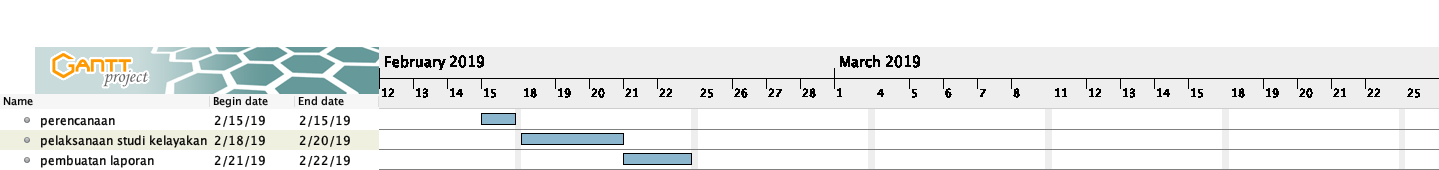
\includegraphics[width=1\textwidth]{./resources/gantt-chart}
	\caption{Grafik \textit{Gantt}}
	\label{fig:002-gantt-chart}
\end{figure}

Karena pengembangan diukur dalam jam, hari, minggu, dan bulan maka kesalahan perkiraan (\textit{error estimation}) yang dibutuhkan untuk perancangan dan implementasi menjadi kecil. Maka nilainya 8.0

\end{enumerate}

Dari keseluruhan faktor kelayakan TELOS tersebut, jumlah dari semua faktornya adalah 

\[ Total = 9 + 9 + 9 + 9 + 8 \]

\[ Total = 44 \]

Total \textit{score} dari kelayakan ini adalah :

\[ score = 44 / 5 = 8,8 \]

Artinya kelayakan sistem komputer yang akan digunakan untuk membangun sistem otentikasi di Badan Pengelolaan Pendataan, Keuangan dan Aset Daerah Kabupaten Brebes adalah LAYAK dengan resiko yang cukup rendah.


\section{SARANA DAN PRASARANA YANG MELIPUTI PERANGKAT KERAS DAN PERANGKAT LUNAK YANG DIPERLUKAN}

Kebutuhan akan sarana dan prasarana untuk jenis perangkat keras yaitu :

\begin{enumerate}
	\item Peladen (\textit{server}) 
	
Peladen atau \textit{server} berfungsi sebagai basis jalannya layanan-layanan aplikasi yang nantinya akan dibangun, nantinya tiap layanan aplikasi akan berjalan pada \textit{container} Docker.

Secara keseluruhan, inti dari aplikasi ini akan berjalan pada 4 (empat) \textit{container}, yang secara ringkas dapat dijelaskan seperti berikut :

\begin{enumerate}

	\item \textit{Container} pertama akan melayani \textit{service} otentikasi, dimana halaman \textit{login} akan berada pada layanan ini, termasuk pemberian token yang digunakan oleh aplikasi klien untuk melakukan akses pada \textit{resource server}. 
	
	\item \textit{Container} kedua berupa layanan basis data yang secara langsung akan terhubung dengan \textit{OAuth Service} atau layanan otentikasi pada \textit{container} pertama dan \textit{resource server}. Dalam layanan basis data ini tersimpan daftar pengguna, hak akses, serta daftar klien yang diijinkan melakukan koneksi ke beberapa \textit{resource server} yang nantinya dibangun.
	
	\item \textit{Container} ketiga berupa layanan dari \textit{resource server} yang nantinya digunakan untuk melakukan pengelolaan baik itu daftar pengguna atau daftar aplikasi klien yang diijinkan untuk terhubung. \textit{Resource server} ini akan berbagi bersama layanan basis data pada \textit{container} kedua dengan layanan \textit{OAuth Server} pada \textit{container} pertama.
	
	\item \textit{Container} keempat berupa layanan aplikasi klien yang berbentuk aplikasi \textit{web}. Aplikasi klien ini akan menggunakan layanan dari \textit{container} pertama, yaitu \textit{OAuth service} sebagai layanan yang akan melakukan otentikasi terhadap pengguna, kemudian atas dasar hak dan kewenangan pengguna yang dapat melakukan akses ke pengelolaan daftar nama pengguna dan daftar aplikasi klien, mampu untuk melakukan akses ke \textit{resource server}, apabila pengguna tidak memiliki hak dan kewenangan tersebut, maka layanan terhadap \textit{resource server} secara sistematis akan ditolak.
	
\end{enumerate}

Kebutuhan perangkat keras peladen (\textit{server}) ini tidak perlu membeli karena nantinya akan menggunakan peladen (\textit{server}) yang sudah ada sebagai peladen (\textit{server}) aplikasi \textit{web} yang sudah beroperasi.

	\item Kartu Jaringan

Kartu jaringan digunakan atau terpasang pada peladen (\textit{server}) agar peladen (\textit{server}) dapat terhubung dengan jaringan, baik jaringan LAN (\textit{Local Area Network}) maupun jaringan \textit{internet}. 

Kartu jaringan ini tidak perlu membeli karena sudah terpasang lebih dari 1 (satu) pada tiap peladen (\textit{server}) yang dapat dikonfigurasi secara mandiri seluruhnya.

\end{enumerate}

Melihat kondisi tersebut, kebutuhan perangkat keras secara keseluruhan sebetulnya tidak perlu mengeluarkan biaya tambahan lain karena perangkat-perangkat tersebut sudah tersedia dan cukup untuk mengakomodir berjalannya sistem informasi yang nantinya akan dibangun.


Kemudian, untuk sarana dan prasarana jenis perangkat lunak yang dibutuhkan yaitu :

\begin{enumerate}
	\item Perangkat Lunak Sistem Operasi

Perangkat lunak sistem operasi digunakan sebagai dasar dari seluruh sistem yang akan berjalan diatasnya. Pemilihan sistem operasi ini pun harus dapat memenuhi kriteria stabil dalam melakukan tugasnya sebagai peladen (\textit{server}) untuk rentang waktu 24 jam selama 7 hari berturut-turut.

Tentunya sistem operasi ini sudah terpasang baik pada peladen-peladen (\textit{servers}) yang nantinya akan menjadi peladen (\textit{server}) sistem basis data dan peladen (\textit{server}) aplikasi \textit{web}. Pada peladen (\textit{server}) aplikasi \textit{web} telah terpasang sistem operasi Ubuntu Server 14.04 yang tentu saja, untuk sistem operasi ini berlisensi gratis sehingga kebutuhan akan peladen (\textit{server}) ini tidak perlu mengeluarkan biaya tambahan baik untuk lisensinya maupun pemasangannya.

\item Perangkat Lunak Sistem Basis Data
	
Perangkat lunak basis data digunakan sebagai sistem yang nantinya akan mengatur dan menyimpan data-data pengguna, data-data hak akses untuk tiap pengguna, serta daftar detail dari aplikasi klien yang diijinkan untuk melakukan akses terhadap \textit{resource server}. 

Pemilihan perangkat lunak basis data ini didasarkan pada lisensinya yang tersedia gratis, namun tidak mengurangi performa dan kehandalannya sebagai tempat simpanan data, sehingga pilihan jatuh pada sistem basis data Postgresql.

Sistem basis data ini sudah lebih dari 30 Tahun dikembangkan dengan lebih dari 400 kontributor, fiturnya pun tidak kalah dengan sistem basis data yang dikembangkan oleh industri-industri besar pada bidang sistem basis data.

Nantinya sistem basis data ini akan berada dalam salah satu \textit{container} docker yang melakukan simpanan data untuk seluruh pengguna berikut hak aksesnya, basis data ini pun nantinya digunakan untuk menyimpan data atau informasi mengenai aplikasi klien yang mampu terhubung dan menggunakan sistem otentikasi yang akan dibangun.

Karena gratis, maka untuk menggunakan sistem basis data Postgresql ini tidak perlu mengeluarkan biaya tambahan untuk pengadaannya.

	\item Perangkat Lunak Peladen \textit{Web}
	
Perangkat lunak peladen (\textit{server}) \textit{web} digunakan untuk menjalankan atau menyediakan aplikasi \textit{web} yang telah dibangun, yaitu sistem otentikasi di Badan Pengelolaan Pendapatan, Keuangan dan Aset Daerah Kabupaten Brebes.

Peladen (\textit{server}) \textit{web} ini nantinya akan ada 2 (dua) macam, yaitu yang berbentuk \textit{web container} yang nantinya digunakan oleh \textit{OAuth Service} dan \textit{Resource Service}, dan yang lain adalah \textit{web server} seperti pada umumnya yang akan melayani aplikasi klien yang telah dibangun.

Untuk peladen (\textit{server}) \textit{web} yang berbentuk \textit{web container} sebetulnya sudah ada dalam satu paket proyek yang dibangun menggunakan \textit{framework} Spring Boot, nantinya paket proyek ini akan dimasukkan dalam sebuah \textit{container} docker, sehingga proses \textit{deployment} akan lebih mudah dengan model \textit{Continuous Integration} dan \textit{Continuous Deployment}.

Alasan kenapa dipilih peladen yang mendukung \textit{servlet} atau \textit{web container} karena memiliki beberapa kelebihan seperti berikut ini :

	\begin{enumerate}
		\item Efisien dan baik dalam \textit{performance}
		
\textit{Performance servlet} dapat dikatakan efisien dan baik karena tidak ada proses pembuatan berulang untuk tiap \textit{request} dari klien (\textit{client}). Setiap \textit{request} ditangani oleh proses \textit{servlet container}. \textit{Servlet} tidak dibuat dan dihancurkan secara berulang-ulang, melainkan tetap tersimpan pada memori untuk menangani \textit{request} yang datang selanjutnya.

		\item \textit{Powerful}

\textit{Servlet} memiliki kemampuan yang lengkap antara lain mampu melakukan penanganan \textit{request}, \textit{session}, \textit{cookie}, akses ke basis data dengan \textit{Java Database Connection} (JDBC) dan \textit{caching}, serta pustaka yang lengkap untuk pembuatan aplikasi \textit{web}.
	
		\item Aman
		
\textit{Servlet} memiliki fasilitas \textit{security} atau keamanan yang baik dan merupakan bagian dari teknologi Java yang sudah dari asalnya didesain dengan \textit{security} atau keamanan yang baik.		
		
		\item Portabilitas
		
Teknologi Java \textit{servlet} dapat dijalankan di berbagai \textit{servlet container, application server}, maupun sistem operasi.		
		
		\item Proses \textit{development} yang lebih cepat
		
Dengan menggunakan \textit{servlet}, kita dapat menggunakan pustaka Java yang lengkap dan menggunakan komponen yang sudah ada tanpa membangun dari awal kembali.		
		
		\item Tangguh
		
\textit{Servlet} merupakan teknologi Java yang memiliki penanganan \textit{memory} yang baik dan \textit{garbage collector} sehingga menjadikan aplikasi \textit{web} yang tangguh dan stabil.		
		
		\item Telah digunakan dan diakui di dunia
		
\textit{Servlet} merupakan teknologi Java yang telah digunakan di berbagai belahan dunia. Dapat ditemukan berbagai komponen, solusi, dan dukungan yang ditawarkan baik secara gratis maupun komersial.		
		
		\item Murah
		
Dikatakan murah karena JDK Java dapat diunduh secara gratis, begitupun dengan \textit{servlet container}.		
		
	\end{enumerate}
	
Pemilihan perangkat lunak peladen (\textit{server}) \textit{web} yang mendukung \textit{servlet} ini pun tidak perlu mengeluarkan biaya, cukup menggunakan Apache Tomcat atau Jetty yang memberikan lisensi gratis dalam penggunaannya, dengan konfigurasi yang tepat, maka peladen (\textit{server}) \textit{web} Apache Tomcat ini cukup untuk melayani permintaan aplikasi dari beberapa klien sekaligus. Sehingga untuk pengadaan perangkat lunak peladen (\textit{server}) \textit{web} ini pun tidak memerlukan tambahan biaya, dan sudah ada dalam paket \textit{framework} Spring Boot untuk kemudahan \textit{debugging} dan \textit{deployment}.

Perangkat lunak peladen (\textit{server}) yang digunakan untuk aplikasi klien nantinya akan menggunakan Nginx yang juga tersedia secara gratis dan sudah teruji kehandalannya karena beberapa perusahaan teknologi informasi besar pun menggunakan Nginx sebagai \textit{web server}-nya.

Ketiga peladen (\textit{server}) ini akan ditempatkan pada masing-masing docker \textit{container} untuk memberikan layanan sesuai dengan tugas dan fungsinya.

	\item Perangkat Lunak Desain Aplikasi
	
Perangkat lunak desain aplikasi digunakan untuk membuat desain pembangunan aplikasi, mulai dari desain struktur basis data, desain \textit{Unified Modeling Language} (UML) yang digunakan untuk membuat spesifikasi standar untuk mendokumentasikan, menspesifikan, dan membangun sistem perangkat lunak, desain UML sendiri dapat menggambarkan atau memodelkan diagram struktur aplikasi dan diagram sifat atau cara kerja aplikasi.

Perangkat lunak atau desain aplikasi ini pun tidak perlu mengeluarkan biaya tambahan, ada perangkat lunak untuk desain aplikasi yang gratis dan disediakan secara daring oleh \href{https://www.draw.io}{https://www.draw.io}. Aplikasi ini memiliki fasilitas yang cukup banyak dan bukan hanya untuk membuat desa UML saja, melainkan desain dari struktur basis data pun mampu dilakukan, kemudian desain jaringan komputer pun dapat dilakukan di aplikasi ini.

	\item Perangkat Lunak \textit{Integrated Development Environment} (IDE)
	
Perangkat lunak IDE ini digunakan untuk membangun aplikasi \textit{web}, baik dari sisi tampilan tatapmuka pengguna (\textit{user interface}) maupun dari sisi kode. Pengujian \textit{unit testing} pun dapat dilakukan dengan menggunakan perangkat lunak ini.

Beberapa pilihan untuk perangkat lunak IDE ini pun beragam dan banyak yang menyediakan secara gratis. Sebagai contoh adalah Netbeans dan Eclipse. Untuk pengembangan aplikasi ini dipilih Intellij IDEA sebagai perangkat dalam membangun layanan \textit{OAuth Service} dan \textit{Resource Service} karena tersedianya beragam \textit{plugins} sebagai pendukung dalam membangun sebuah aplikasi, sedangkan untuk membangun aplikasi klien yang digunakan untuk melakukan pengelolaan atau manajemen pengguna dan aplikasi klien lain, akan menggunakan Visual Studio Code, karena pada Visual Studio Code ini pun terdapat beragam \textit{plugins} yang mampu mendukung dan mempermudah pengerjaan aplikasi klien nantinya.

Kedua aplikasi itu, baik Intellij IDEA dalam hal ini, yang digunakan adalah versi komunitas (\textit{community edition}) dan Visual Studio Code tersedia secara gratis dan bebas diunduh dari masing-masing laman penyedianya, sehingga untuk pengadaan perangkat lunak IDE ini tidak perlu mengeluarkan biaya tambahan.

		\item Perangkat Lunak Docker
		
		Perangkat lunak docker ini digunakan untuk membangun \textit{container-container} kecil yang nantinya berjalan secara independen yang tiap \textit{container}-nya akan menjalankan sebuah layanan (\textit{service}) tertentu yang spesifik, contohnya, sebuah \textit{container} hanya akan menjalankan layanan (\textit{service}) basis data saja, sedangkan \textit{container} yang lain hanya akan menjalankan layanan (\textit{service}) \textit({OAuth Service}), keduanya akan berjalan secara independen dan paralel yang apabila ingin kedua layanan atau \textit{container} ini saling terhubung, akan melalui sebuah sambungan yang didefinisikan secara khusus.
		
		Bisa diistilahkan bahwa docker ini adalah bentuk virtualisasi yang lebih ringan, karena sebetulnya, didalam sebuah \textit{container} akan terdapat sebuah sistem operasi yang berjalan, serta beberapa aplikasi pendukung yang tujuannya spesifik untuk menjalankan layanan (\textit{service}) utamanya. Contohnya, saat ada \textit{container} yang memiliki layanan (\textit{service}) basis data Postgresql, maka disana akan terdapat sebuah sistem operasi, basis data Postgresql, dan beberapa pustaka pendukung agar basis data Postgresql dapat berjalan.
		
		Untuk penggunaan docker ini kita pun dapat memilih menggunakan versi \textit{Enterprise} atau \textit{community edition}, untuk membangun aplikasi ini, sebetulnya kebutuhan untuk menggunakan versi \textit{community edition} sudah cukup, sehingga kita tidak memerlukan biaya tambahan lain untuk mendapatkannya.
		
		\item Perangkat Lunak Git
		
		Perangkat lunak Git digunakan untuk melakukan \textit{Continuous Integration} dengan lebih sempurna. Fungsi dari perangkat lunak Git ini sebetulnya tergolong dalam aplikasi \textit{Versioning Control} yang melakukan pencatatan atau \textit{log} dari kondisi perubahan berkas atau kandar, sehingga saat melakukan perubahan-perubahan yang terjadi pada fitur aplikasi yang dibangun dapat dilihat historis perubahannya, dan apabila ada kesalahan implementasi fitur dan perlu untuk dikembalikan kondisi ke beberapa keadaan diwaktu sebelumnya, mampu dilakukan dengan mudah tanpa harus mengubah kondisi berkas saat ini.
		
		Fungsi lain dari perangkat lunak Git ini sebetulnya adalah untuk kebutuhan kolaborasi, dimana 1 (satu) atau lebih pengkode (\textit{coder}) dapat mengerjakan pekerjaan koding (\textit{coding}) secara bersama-sama dan paralel, setelah perkerjaan satu sub-modul atau sebuah fitur selesai, hasil kodenya dapat digabung sehingga menjadi satu fitur yang lengkap dan dapat digunakan.
		
		Penggunaan Git ini tidak terlepas dari sebuah peladen (\textit{server}) Git yang digunakan untuk mengumpulkan seluruh hasil penetapan (\textit{commit}) kode dari masing-masing pengkode (\textit{coder}), yang digunakan nantinya sebagai peladen (\textit{server}) Git adalah Gitlab, karena disana sudah terdapat fitur \textit{Continuous Deployment} (CD) yang berfungsi untuk melakukan instalasi atau pemasangan secara otomatis pada peladen (\textit{server}) VPS milik unit kerja Badan Pengelolaan Pendapatan, Keuangan dan Aset Daerah.
		
		Pada proses \textit{Continuous Integration} dan \textit{Continuous Deployment} (CI/CD) nantinya, dapat dilakukan konfigurasi fase penyelarasan kode yang dapat diatur sesuai kebutuhan, contohnya, pada saat kode dari tiap pengkode (\textit{coder}) akan digabung, maka otomatis akan melakukan \textit{unit test} untuk memastikan bahwa tidak ada kesalahan logika program per sub-unit kode terkecil sekaligus melakukan \textit{integration test} untuk memastikan bahwa fitur baru atau pembersihan \textit{bugs} yang dilakukan tidak bermasalah apabila sistem berada pada lingkungan yang mengharuskannya terhubung ke beberapa sumber daya (\textit{resource}) seperti sistem basis data, jaringan, atau hal lain yang dibutuhkan sistem untuk melakukan kegiatan operasionalnya.
		
		Penggunaan Git dapat diperoleh dan diunduh dengan gratis dari \href{https://git-scm.com/}{https://git-scm.com/}, sedangkan Gitlab sendiri menyediakan layanannya dalam beberapa versi sesuai kebutuhan, dan fitur CI/CD yang kita butuhkan sudah ada pada versi gratis yang ditawarkan oleh layanan ini, sehingga tidak perlu mengluarkan biaya untuk menggunakan layanan dari GItlab ini.

	\item Kotlin \textit{Compiler}

\textit{Compiler} ini digunakan untuk melakukan kompilasi kode yang ditulis dengan bahasa pemrograman Kotlin. Pemilihan bahasa pemrograman Kotlin ini sebagai dasar pembangunan aplikasi atau sistem Otentikasi karena mampu bersinergi dengan sistem yang dibangun menggunakan bahasa Java, dengan kata lain, karena \textit{framework} yang digunakan adalah Spring Boot yang dibangun menggunakan bahasa pemrograman Java, penggunaan bahasa pemrograman Kotlin dengan menggunakan \textit{framework} Spring sangat memungkinkan dengan ditambah kehandalan dari bahasa pemrograman Kotlin yang mampu mendeteksi atau mengurangi timbulnya \textit{Null Exception} pada aplikasi.

Kotlin \textit{Compiler} sendiri tersedia secara gratis dan dapat diunduh dari lamah \href{https://kotlinlang.org/}{https://kotlinlang.org/}, sehingga penggunaannya tidak memerlukan biaya tambahan.

	\item Maven

Maven digunakan sebagai \textit{build-tools} untuk mempermudah pengelolaan proyek yang akan dibangun, untuk menggunakan berbagai macam pustaka seperti diatas, cukup dideklarasikan pada sebuah berkas konfigurasi Maven dengan nama \texttt{pom.xml}, untuk melakukan pemaketan (\textit{packaging}) pun sangat mudah, nantinya dengan Maven, sebelum sebuah proyek didistribusikan atau di \textit{deploy} ke peladen (\textit{server}), akan dilakukan serangkaian tes (\textit{unit test} dan \textit{integration test}) untuk memastikan bahwa kode yang dibangun telah memenuhi kelayakan untuk digunakan.

\end{enumerate}

\section{SUMBER DAYA MANUSIA YANG TERLIBAT DALAM SISTEM KOMPUTER}

Penentuan sistem komputer yang layak untuk digunakan tidak terlepas dari Sumber Daya Manusia, adapun Sumber Daya Manusia (SDM) yang terlibat dalam penentuan kelayakan sistem komputer yang akan digunakan sebagai peladen (\textit{server}) dari sistem otentikasi yang akan dibangun adalah seorang Fungsional Pranata Komputer yang secara kemampuan memiliki kompetensi untuk melakukan studi kelayakan sistem komputer ini.

\section{WAKTU DAN BIAYA YANG DIBUTUHKAN DALAM PEMBUATAN / PENGEMBANGAN SISTEM APLIKASI SECARA MENYELURUH}

Dari sisi biaya, maka tidak diperlukan pengeluaran biaya untuk pembuatan / pengembangan ini, karena sebetulnya seluruh perangkat keras sudah terpasang dan berjalan normal, dan dari pengadaan perangkat lunaknya pun semuanya menggunakan versi gratis.

Sedangkan dari waktu yang dibutuhkan, akan menghabiskan waktu sekitar 1 (satu) minggu yang tentu saja ini waktu yang tidak terlalu lama untuk menentukan kelayakan sebuah sistem komputer yang akan digunakan.

\end{document}
